\section{Experiments}\label{sec:experiments}
% Every number below is produced by a named script in the empirical directory (heracles-emp):
%   REG  = preregistered analysis, experiments/E*/REPORT.md;
%   A1/A2 = post-hoc amendments, experiments/common/amend_A1.py, amend_A2_shape.py (AMENDMENTS.md in each experiment);
%   figures and caption numbers: paper_figs/make_figs.py -> paper_figs/FIGURE_NUMBERS.json;
%   audit of all of the above: AUDIT.md (its section 6 lists the statements used here).

We train the networks of Section~\ref{sec:prelim} with full-batch gradient descent with momentum and ask whether the number of features tracks the programme \eqref{eq:programme}. Theorem~\ref{thm:cyclic} is a statement about interference-free maximizers. Yet trained networks are neither interference-free nor exact maximizers, hence, we predict trends in the number of frequencies observed and not exact counts. Training details, the convergence criterion and the count definition are in Appendix~\ref{app:exp}.

\subsection{Where interference enters trained networks}

Trained networks carry some interference: most of their logit energy lies in the clean modes $(j,\dots,j;-j)$ (median $0.97$), and less of it as $s$ grows. They are also not maximizers of the programme. Their learned allocations reach about $0.87$ of the optimum $\Gamma_s(p)$, well above a random allocation or the network at initialization, but the individual budget shares do not match $y^*$. No trained network exceeded the universal bound of Theorem~\ref{thm:universal}. The numbers behind this section are in Appendix~\ref{app:exp}.

\subsection{The exponent \texorpdfstring{$s=\nu/b$}{s = nu/b}}

\begin{figure}[t]
\centering
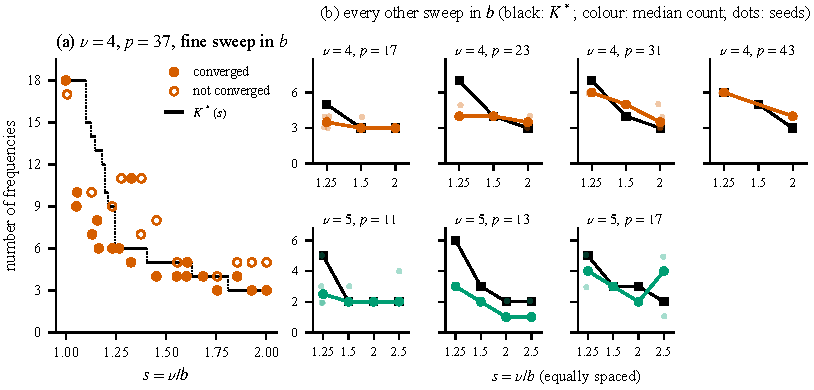
\includegraphics[width=\linewidth]{figures/fig_exponent.pdf}
\caption{\textbf{The count follows the exponent.} (a) Product networks at $\nu=4$, $p=37$, sweeping $b$ from $4$ to $2$ ($s$ from $1$ to $2$). Black: $\Kstar(s)$, exact, with its twelve plateaus (the two at $\Kstar=6$ differ in their amplitude ratios). Each marker is one run ($19$ converged, $13$ not). (b) Every other sweep in $b$ at fixed $(\nu,p)$ with at least two converged cells ($\nu=4$, $p=59$, where $8$ of $12$ runs diverged, has one and is omitted). Black: $\Kstar$; colour: median count over converged seeds; dots: individual seeds. The $s$ values are drawn equally spaced.}
\label{fig:exponent}
\end{figure}

Sweeping the norm exponent at fixed degree and prime (Figure~\ref{fig:exponent}a), the trained count falls with $\Kstar$, from every frequency at $b=\nu$ to three at $b=2$, although it does not resolve the finer plateaus of $\Kstar$. The same holds in every other sweep in $b$ (Figure~\ref{fig:exponent}b and, at $\nu=3$, Figure~\ref{fig:prime}). Across all pairs of settings that share $\nu$ and $p$ but differ in $b$, the trained count moves in the same direction as $\Kstar$ in $30$ of $36$ (Appendix~\ref{app:exp}).

At the dense end, $b=\nu$ ($s=1$, the left end of Figure~\ref{fig:exponent}a), every converged network at $\nu=3$ and $\nu=4$ uses every frequency, most with near-equal amplitudes, as Corollary~\ref{cor:dense} predicts; density alone is not diagnostic, since the network at initialization is already dense, but flatness is. At $\nu=5$ the picture is mixed.

\subsection{Moving the degree and the norm separately}

Theorem~\ref{thm:cyclic} says that the optimal spectral allocation depends on $\nu$ and $b$ only through $s$. At equal $s$, trained networks of different degree use the same number of frequencies to within one in $12$ of $17$ comparisons: gradient descent falls further below $\Kstar$, and further from the optimum, as the degree grows (Appendix~\ref{app:exp}).

\begin{figure}[h!]
\centering
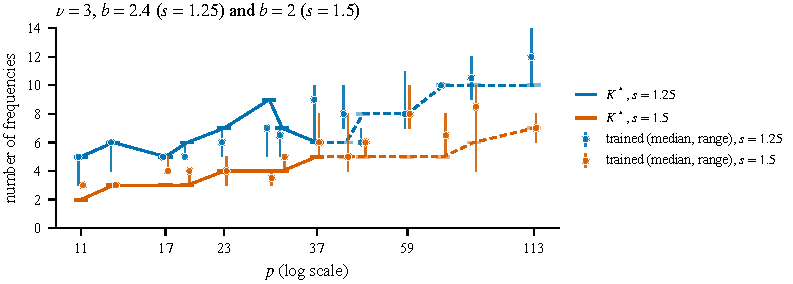
\includegraphics[width=\linewidth]{figures/fig_prime.pdf}
\caption{\textbf{The count across primes}, product networks at $\nu=3$. Lines: $\Kstar$ (solid where exact, $p\le37$; dashed where best found, Appendix~\ref{app:exp}). Markers: median over converged seeds, with the range. $\Kstar$ is not monotone in $p$ (at $s=1.25$ it is $9,7,6$ at $p=29,31,37$); the trained counts do not follow these steps.}
\label{fig:prime}
\end{figure}

Across primes (Figure~\ref{fig:prime}), the count stays within one of $\Kstar$ in most $(p,s)$ cells ($20$ of $28$, against $16$ for the best constant), but it does not follow the non-monotone steps of $\Kstar$.

\FloatBarrier
